%=========================================================================================================
\section{Introduction}
\label{sec:introduction}
%=========================================================================================================

%--- 1.1 Continual AD Problem Definition ---

Industrial anomaly detection (AD) has become indispensable for quality control in modern manufacturing. Deep learning approaches, particularly those based on normalizing flows~\citep{dinh2016realnvp,gudovskiy2022cflow}, memory banks~\citep{roth2022patchcore}, and reconstruction~\citep{zavrtanik2021draem}, have achieved remarkable success by learning density models of normal samples. However, these methods implicitly assume a static deployment scenario: train once on a fixed set of product categories, then deploy indefinitely.

Real-world manufacturing environments violate this assumption. Production lines evolve---new products (e.g., transistors) are introduced alongside existing ones (e.g., capacitors, cables), data privacy regulations may prohibit storing historical samples, and edge devices impose strict memory constraints. Under these conditions, models must learn \emph{continually}: acquiring knowledge of new product categories while retaining detection capability for previously learned ones. The central challenge is \textbf{catastrophic forgetting}~\citep{kirkpatrick2017ewc}---when training on task $t$ overwrites the representations learned for tasks $0, \ldots, t-1$, performance on earlier tasks degrades catastrophically:
\begin{equation}
\text{Forgetting} = \frac{1}{t}\sum_{i=0}^{t-1} \left( \text{AUROC}^{(i)}_{\text{after } i} - \text{AUROC}^{(i)}_{\text{after } t} \right) \gg 0
\label{eq:forgetting}
\end{equation}

%--- 1.2 The Isolation-Efficiency Dilemma ---

At its core, continual learning faces a fundamental tension that we term the \textbf{Isolation-Efficiency Dilemma}:

\begin{itemize}
    \item \textbf{Parameter Isolation} ensures zero forgetting: if task-specific parameters are completely separated, training on new tasks cannot interfere with previous knowledge. The extreme case---maintaining a full model copy per task---achieves perfect isolation but incurs $O(N \times P)$ memory cost for $N$ tasks with $P$ parameters each, rendering it impractical.

    \item \textbf{Parameter Efficiency} enables scalability: sharing parameters across tasks maintains $O(P)$ memory regardless of task count, but shared parameters are susceptible to overwriting, causing forgetting.
\end{itemize}

This dilemma is not merely a practical inconvenience but a structural constraint that has shaped the entire landscape of continual learning research. Existing methods navigate this trade-off through various compromises, each sacrificing either isolation or efficiency to some degree.

%--- 1.3 Existing Methods: A History of Compromise ---

\textbf{Regularization-based methods} (EWC~\citep{kirkpatrick2017ewc}, LwF~\citep{li2017lwf}) constrain parameter updates based on importance metrics, but the regularization strength must balance plasticity for new tasks against stability for old ones. This inherent trade-off yields non-zero forgetting (typically 3--5\% on MVTec AD) that accumulates across tasks.

\textbf{Replay-based methods} store exemplars from previous tasks to rehearse during new task training. While effective, they introduce memory overhead proportional to buffer size, raise data privacy concerns, and suffer from representation bias toward stored samples. Moreover, for density estimation tasks like anomaly detection, replayed samples may not adequately preserve the tail regions critical for boundary modeling.

\textbf{Dynamic architecture methods} (PackNet~\citep{mallya2018packnet}, Progressive Networks~\citep{rusu2016progressive}) allocate dedicated network capacity per task through pruning or expansion. However, binary masks lack flexibility, capacity saturates as tasks accumulate, and the overhead grows linearly with task count.

\textbf{Prompt/Adapter methods} (L2P~\citep{wang2022learning}, DualPrompt~\citep{wang2022dualprompt}) freeze pretrained backbones and learn task-specific prompts or adapters. While parameter-efficient, these methods optimize for discriminative classification boundaries rather than the precise density estimation required for anomaly detection. The resulting feature space distortions can compromise anomaly scoring fidelity.

%--- 1.4 Our Insight: NF's Arbitrary Function Property Enables Decomposition ---

We propose a fundamentally different approach that achieves \emph{both} complete isolation \emph{and} high efficiency---breaking the dilemma rather than compromising within it. Our key insight emerges from a structural property of normalizing flows that, while known since~\citet{dinh2016realnvp}, has not been exploited for continual learning:

\begin{quote}
\textbf{Design Principle 1 (Invertibility-Independence Decomposition):} In affine coupling layers, the invertibility guarantee depends solely on the coupling structure---the input splitting and affine combination---\emph{not on how the subnet functions $s(\cdot)$ and $t(\cdot)$ are internally parameterized}.
\end{quote}

This principle has profound implications. Unlike VAEs, where encoder and decoder must remain jointly calibrated, or diffusion models, where timestep-conditional denoising creates temporal dependencies, normalizing flow subnets are \emph{structurally unconstrained}. We can freely decompose subnet weights into shared and isolated components:
\begin{equation}
\mathbf{W}_{\text{task}} = \underbrace{\mathbf{W}_{\text{base}}}_{\text{frozen, shared}} + \underbrace{\frac{\alpha}{r}\mathbf{B}_t\mathbf{A}_t}_{\text{task-specific, isolated}}
\label{eq:decomposition}
\end{equation}
without compromising invertibility, exact likelihood computation, or any theoretical guarantee of the normalizing flow.

%--- 1.5 Parameter Decomposition Strategy ---

Building on this insight, we propose \textbf{MoLE-Flow} (Mixture of LoRA Experts for Normalizing Flow), a framework that decomposes coupling subnet parameters into:
\begin{itemize}
    \item \textbf{Frozen shared base weights} $\mathbf{W}_{\text{base}}$: learned on Task 0 and frozen thereafter, encoding the canonical transformation from feature space to standard Gaussian.
    \item \textbf{Isolated task-specific LoRA adapters} $\{(\mathbf{A}_t, \mathbf{B}_t)\}$: low-rank matrices that modulate the base transformation for each task's specific distribution characteristics.
\end{itemize}

This decomposition achieves \textbf{zero forgetting by design}---not through regularization or replay, but through architectural isolation. Since each task's LoRA adapters are completely independent, training task $t$ cannot modify the adapters of any previous task. Simultaneously, the low-rank constraint ensures \textbf{parameter efficiency}: with rank $r=64$, each task adds only $\sim$8\% of base model parameters, yielding $O(P + N \times r)$ scaling.

%--- 1.6 Base Freeze Side Effects and Integral Components ---

While base freezing guarantees isolation, it introduces structural rigidity that manifests as three specific side effects:

\begin{enumerate}
    \item \textbf{Input Interface Mismatch}: The frozen base expects input distributions similar to Task 0. New tasks with different feature statistics create a distribution mismatch that LoRA alone cannot efficiently resolve.

    \item \textbf{Gradient Concentration at Bulk}: LoRA makes incremental adjustments to a fixed transformation. Standard likelihood training concentrates gradients on the abundant ``easy'' samples near the distribution center, under-training the critical boundary (tail) regions.

    \item \textbf{Global Transformation Rigidity}: The frozen base captures only global transformation structure. Local, high-frequency patterns (e.g., fine textures in screws, subtle cable surface defects) exceed the representational scope of low-rank perturbations.
\end{enumerate}

To compensate for these side effects, we introduce three \textbf{Integral Components}---modules that are not generic performance boosters but rather \emph{structurally necessary} under the frozen-base regime:
\begin{itemize}
    \item \textbf{WhiteningAdapter (WA)}: Performs task-specific affine distribution alignment \emph{before} the flow, enabling LoRA to focus on nonlinear pattern adaptation rather than distribution correction.
    \item \textbf{Tail-Aware Loss (TAL)}: Upweights high-loss (tail) samples during training, redistributing gradients toward boundary regions critical for anomaly detection.
    \item \textbf{Deep Invertible Adapter (DIA)}: Appends task-specific invertible coupling blocks \emph{after} the base flow, providing residual local corrections for high-frequency patterns.
\end{itemize}

%--- 1.7 Methodological Contribution: Interaction Effect Analysis ---

A potential criticism is that these components might be ``bags of tricks'' that improve any model rather than targeted compensations for base freezing. We address this through a novel \textbf{Interaction Effect Analysis} framework that distinguishes integral components from generic boosters.

The key insight: if a component is a generic booster, it should provide similar gains regardless of whether the base is trainable or frozen. Conversely, if a component specifically compensates for base freeze side effects, its benefit should be \emph{asymmetric}---large when base is frozen, negligible or even harmful when base is trainable.

Our analysis reveals precisely this asymmetry:
\begin{itemize}
    \item \textbf{DIA}: Trainable base $\rightarrow \Delta$P-AP = $-3.78\%$ (harmful); Frozen base $\rightarrow \Delta$P-AP = $+4.14\%$ (beneficial)
    \item \textbf{TAL}: Trainable base $\rightarrow \Delta$P-AP = $+5.10\%$; Frozen base $\rightarrow \Delta$P-AP = $+7.52\%$ (1.47$\times$ larger)
\end{itemize}

The DIA result is particularly striking: the same component that \emph{degrades} performance with a trainable base \emph{improves} it with a frozen base. This provides strong evidence that DIA addresses a specific limitation introduced by base freezing---global transformation rigidity---rather than providing generic enhancement.

%--- 1.8 Contributions ---

In summary, we make the following contributions:

\begin{itemize}
    \item \textbf{Structural Connection.} We establish a novel connection between the arbitrary function property of normalizing flow coupling layers and the parameter decomposition requirements of continual learning. This connection, overlooked by prior work due to the separation between generative modeling and CL research communities, enables zero-forgetting continual learning with $O(N \times r)$ efficiency.

    \item \textbf{Parameter-Efficient Isolation Framework.} We instantiate this insight through MoLE-Flow, decomposing coupling subnets into frozen shared bases and task-specific LoRA adapters, achieving zero forgetting by design with only 8\% parameter overhead per task.

    \item \textbf{Interaction Effect Analysis Framework.} We introduce a methodology for validating whether proposed components are integral to a design choice or generic boosters, by measuring asymmetric effects across different architectural conditions. This framework has broader applicability for component validation in continual learning research.

    \item \textbf{State-of-the-Art Results.} On MVTec-AD (15 classes, 5 runs), MoLE-Flow achieves 98.05$\pm$0.12\% image-level AUROC and 55.80$\pm$0.35\% pixel-level AP with \emph{zero} forgetting, surpassing CADIC by 0.9\% while completely eliminating the forgetting that affects all prior methods.
\end{itemize}

The remainder of this paper is organized as follows. Section~\ref{sec:related_work} reviews related work in anomaly detection, continual learning, and normalizing flows. Section~\ref{sec:method} presents our methodology, beginning with the key insight on parameter decomposition, followed by the MoLE-Flow architecture and integral components. Section~\ref{sec:experiments} provides comprehensive experimental validation, and Section~\ref{sec:conclusion} concludes with discussion of limitations and future directions.


%=========================================================================================================
\section{Proposed Method}
\label{sec:method}
%=========================================================================================================

\begin{figure*}[t]
    \centering
    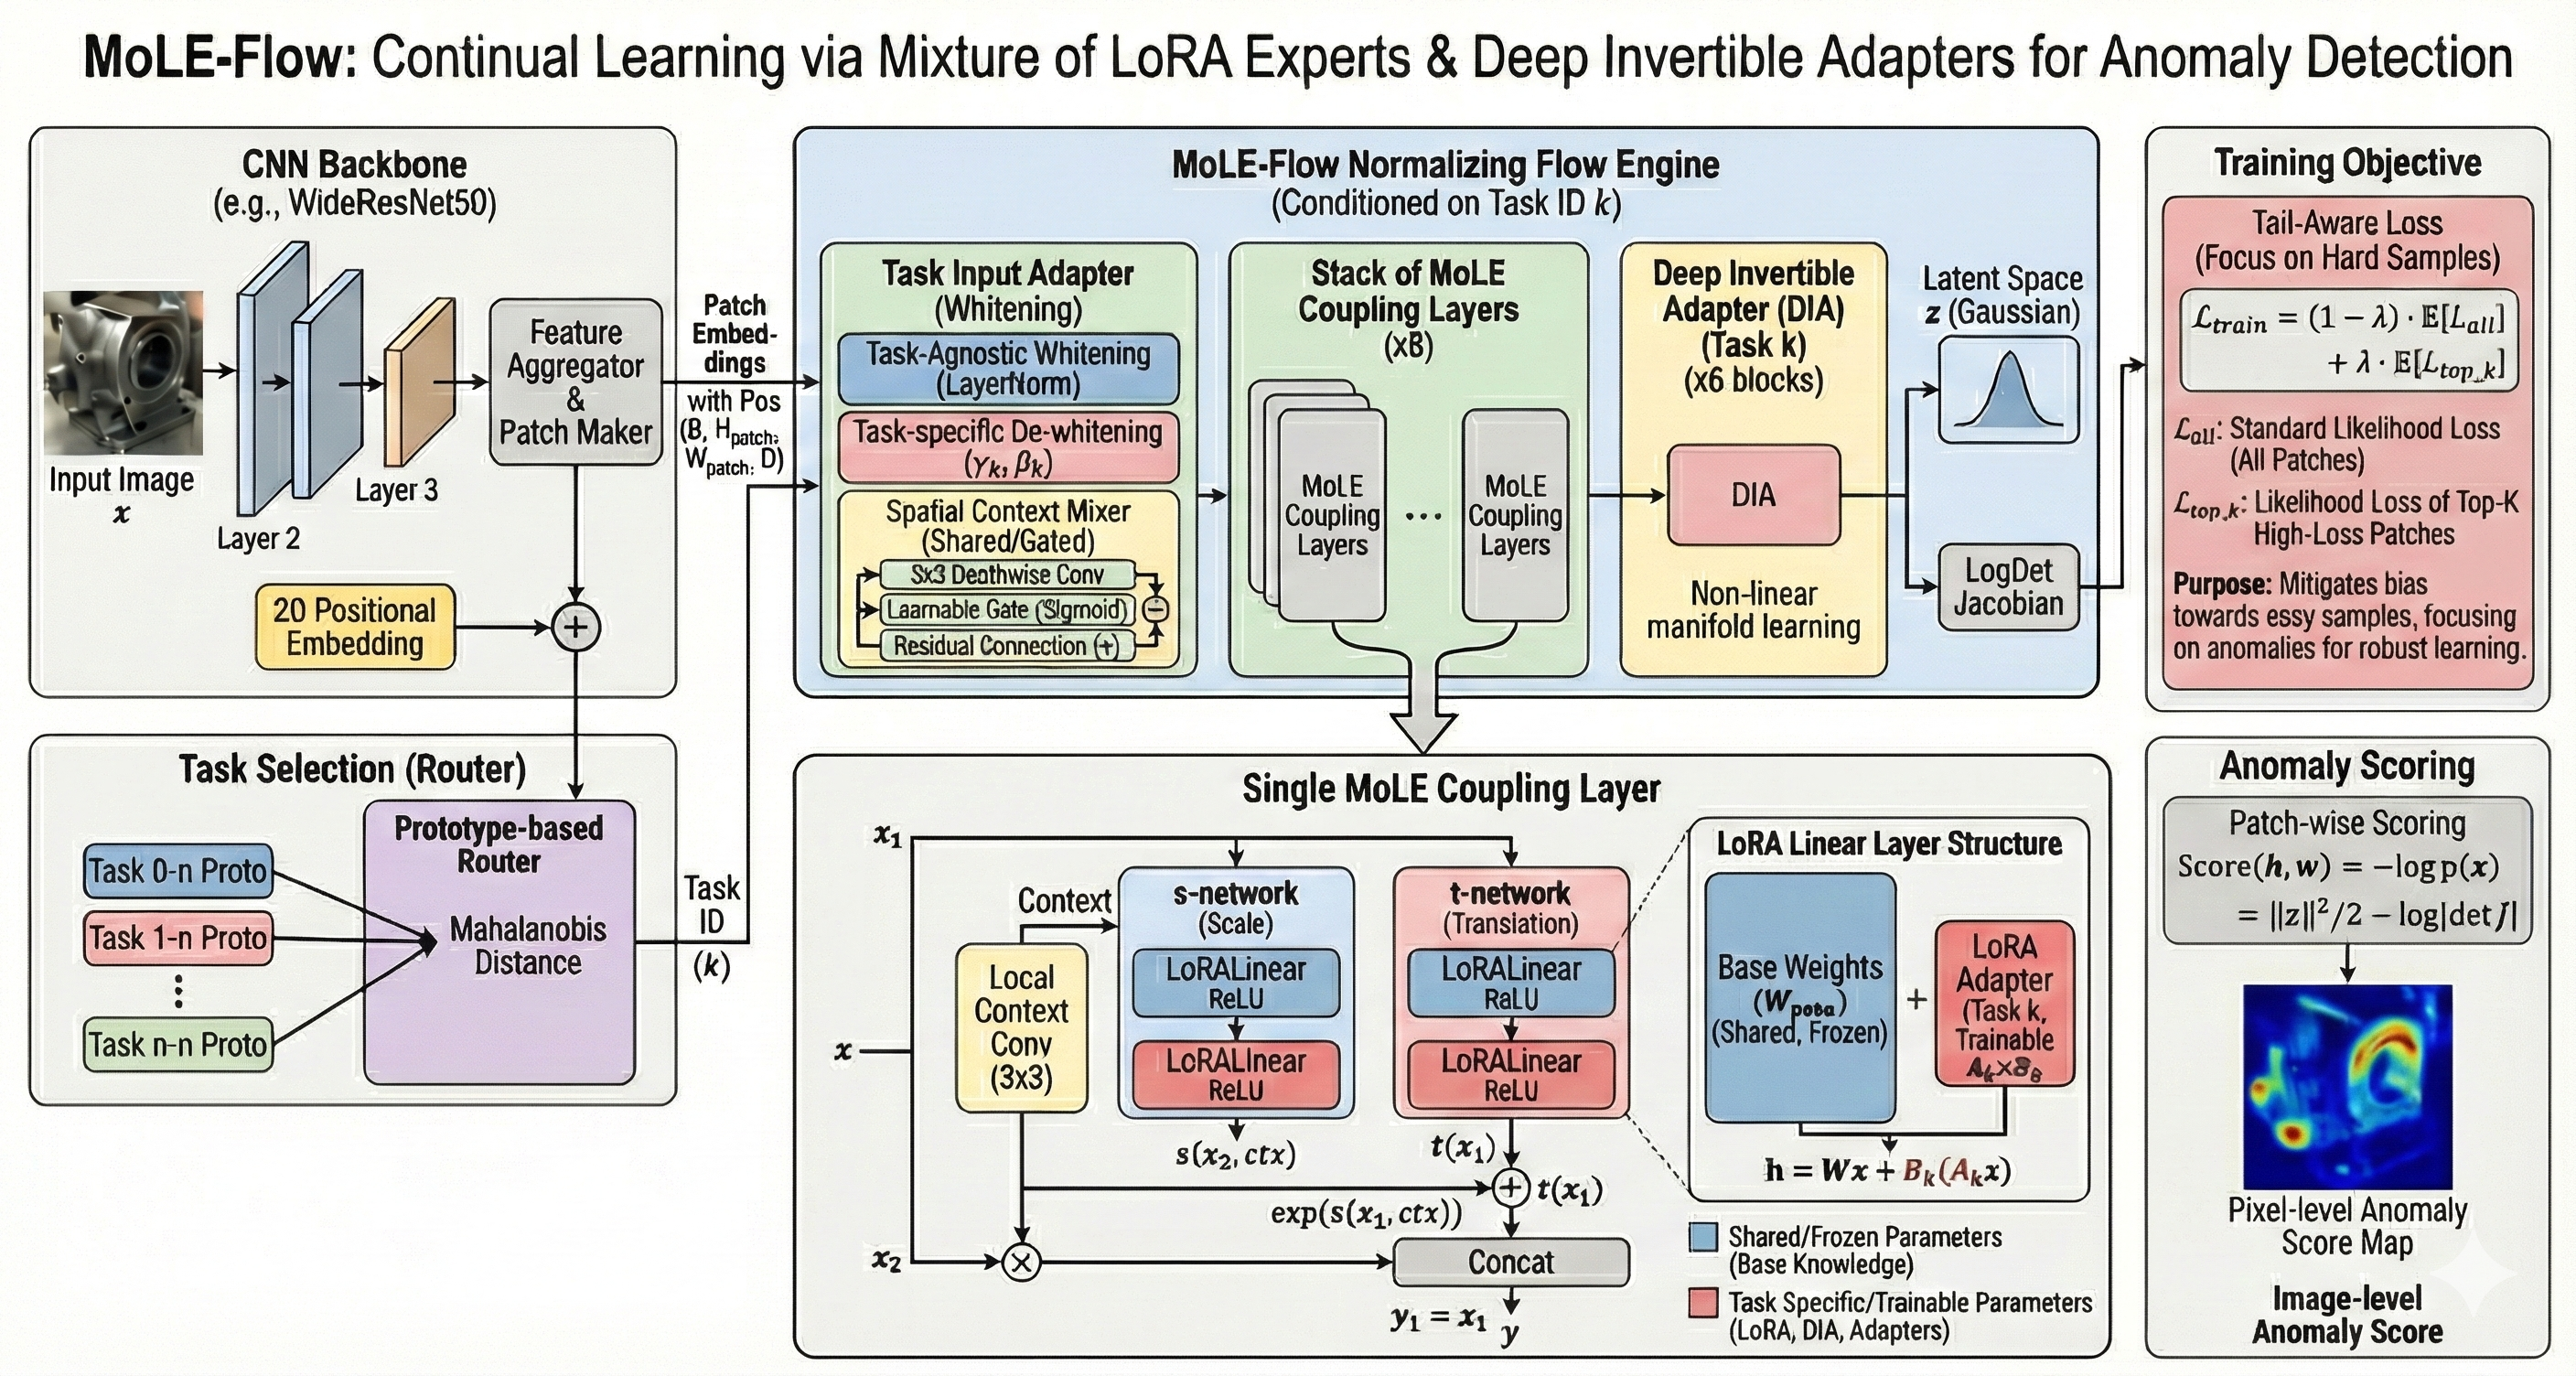
\includegraphics[width=\textwidth]{figures/main2.png}
    \caption{\textbf{MoLE-Flow framework overview.} (a)~The isolation-efficiency dilemma: complete parameter isolation (full model copy) prevents forgetting but incurs $O(N \times P)$ memory; shared parameters are efficient but cause forgetting. (b)~Our solution leverages Design Principle 1: coupling layer invertibility is independent of subnet parameterization, enabling decomposition into frozen shared base plus task-specific LoRA adapters. (c)~Complete architecture showing the frozen base NF, task-specific components (WhiteningAdapter, LoRA, DIA), and prototype-based routing.}
    \label{fig:main_figure}
\end{figure*}

This section presents MoLE-Flow, our framework for resolving the isolation-efficiency dilemma in continual anomaly detection. We begin by examining why parameter decomposition is the only viable solution (Section~\ref{sec:decomposition_necessity}), then establish why normalizing flows are uniquely suited for safe decomposition (Section~\ref{sec:why_nf}). Subsequently, we detail the MoLE-Flow architecture (Section~\ref{sec:architecture}), describe the integral components that compensate for base freeze rigidity (Section~\ref{sec:integral_components}), and present our prototype-based routing mechanism (Section~\ref{sec:routing}).

%=========================================================================================================
\subsection{Parameter Decomposition: The Only Solution}
\label{sec:decomposition_necessity}
%=========================================================================================================

Before detailing our approach, we establish why parameter decomposition is not merely \emph{one} solution but the \emph{only} solution that simultaneously satisfies both isolation and efficiency requirements.

\subsubsection{Two Conditions That Must Be Satisfied}

Continual learning imposes two seemingly contradictory requirements:

\begin{itemize}
    \item \textbf{Isolation Requirement}: Task parameters must not interfere across tasks. Formally, training on task $t$ should not modify any parameters that affect the output for tasks $i < t$.

    \item \textbf{Efficiency Requirement}: Memory should not scale linearly with task count. Formally, total parameters should be $O(P + N \cdot \delta)$ where $\delta \ll P$.
\end{itemize}

\subsubsection{Exhaustive Strategy Analysis}

We exhaustively consider all possible strategies for organizing model parameters across tasks:

\begin{table}[t]
\centering
\caption{Exhaustive analysis of parameter organization strategies for continual learning.}
\label{tab:strategies}
\begin{tabular}{l|cc|c}
\toprule
\textbf{Strategy} & \textbf{Isolation} & \textbf{Efficiency} & \textbf{Assessment} \\
\midrule
Full Model Copy & \ding{51} Complete & \ding{55} $O(N \times P)$ & Impractical \\
Shared Weights & \ding{55} Interference & \ding{51} $O(P)$ & Forgetting \\
\textbf{Decomposition} & \ding{51} \textbf{Delta isolated} & \ding{51} \textbf{$O(P + N \cdot \delta)$} & \textbf{Both satisfied} \\
\bottomrule
\end{tabular}
\end{table}

\textbf{Full Model Copy}: Maintaining separate model instances per task trivially satisfies isolation---each task has its own parameters that cannot be modified by other tasks. However, this incurs $O(N \times P)$ memory, which becomes prohibitive as $N$ grows (e.g., 15 tasks $\times$ 50MB = 750MB for base flow alone).

\textbf{Shared Weights}: All tasks share the same parameters, achieving optimal $O(P)$ memory. However, gradients from task $t$ directly modify parameters used by all previous tasks, causing forgetting. Regularization and replay can \emph{mitigate} but not \emph{eliminate} this interference.

\textbf{Parameter Decomposition}: We decompose weights as:
\begin{equation}
\mathbf{W}_t = \mathbf{W}_{\text{shared}} + \Delta\mathbf{W}_t
\end{equation}
where $\mathbf{W}_{\text{shared}}$ is frozen after initial training and $\Delta\mathbf{W}_t$ is task-specific. Isolation holds because each $\Delta\mathbf{W}_t$ is independent. Efficiency holds if $\Delta\mathbf{W}_t$ can be parameterized with $\delta \ll P$ parameters---achievable via low-rank factorization $\Delta\mathbf{W}_t = \frac{\alpha}{r}\mathbf{B}_t\mathbf{A}_t$.

\textbf{Conclusion}: Parameter decomposition is the unique strategy that satisfies both requirements. The remaining question is: which model architectures permit such decomposition \emph{safely}?

%=========================================================================================================
\subsection{Model Comparison: Why Normalizing Flow Enables Safe Decomposition}
\label{sec:why_nf}
%=========================================================================================================

Not all generative models can accommodate parameter decomposition without compromising their core functionality. We analyze three prominent density estimation architectures.

\subsubsection{VAE: Encoder-Decoder Coupling Breaks}

Variational Autoencoders jointly optimize an encoder $q_\phi(\mathbf{z}|\mathbf{x})$ and decoder $p_\theta(\mathbf{x}|\mathbf{z})$ through the ELBO:
\begin{equation}
\mathcal{L}_{\text{ELBO}} = \mathbb{E}_{q_\phi}[\log p_\theta(\mathbf{x}|\mathbf{z})] - D_{\text{KL}}(q_\phi(\mathbf{z}|\mathbf{x}) \| p(\mathbf{z}))
\end{equation}

The encoder and decoder are \emph{structurally coupled}---the decoder is optimized to reconstruct from latent codes produced by the encoder. If we insert adapters only in the encoder, the decoder receives latent codes from a modified distribution that it was not trained to decode. Inserting adapters in both encoder and decoder requires careful synchronization to maintain latent space coherence---a fragile arrangement prone to failure modes.

\subsubsection{Diffusion: Sampling Path Distortion}

Diffusion models learn a denoiser $\epsilon_\theta(\mathbf{x}_t, t)$ that operates across hundreds of timesteps during sampling:
\begin{equation}
\mathbf{x}_{t-1} = \frac{1}{\sqrt{\alpha_t}}\left(\mathbf{x}_t - \frac{1-\alpha_t}{\sqrt{1-\bar{\alpha}_t}}\epsilon_\theta(\mathbf{x}_t, t)\right) + \sigma_t \mathbf{z}
\end{equation}

Modifying the denoiser at any timestep affects all subsequent sampling steps. The effect of an adapter inserted at timestep $t$ propagates and compounds through all steps $t-1, t-2, \ldots, 0$, making it difficult to predict or control the final output. Moreover, exact likelihood computation requires expensive probability flow ODEs, complicating analysis.

\subsubsection{Normalizing Flow: Arbitrary Function Property Preserves Guarantees}

Normalizing flows transform data through a sequence of invertible mappings. The affine coupling layer~\citep{dinh2016realnvp} has the form:
\begin{align}
\mathbf{y}_1 &= \mathbf{x}_1 \label{eq:coupling_y1} \\
\mathbf{y}_2 &= \mathbf{x}_2 \odot \exp(s(\mathbf{x}_1)) + t(\mathbf{x}_1) \label{eq:coupling_y2}
\end{align}
with inverse:
\begin{align}
\mathbf{x}_1 &= \mathbf{y}_1 \label{eq:coupling_inv_x1} \\
\mathbf{x}_2 &= (\mathbf{y}_2 - t(\mathbf{y}_1)) \odot \exp(-s(\mathbf{y}_1)) \label{eq:coupling_inv_x2}
\end{align}

The critical observation is that invertibility is guaranteed by the \emph{coupling structure}---the input splitting and element-wise affine combination---\textbf{regardless of how $s(\cdot)$ and $t(\cdot)$ are implemented}. The subnet functions can be MLPs, convolutions, transformers, or any parameterization; the flow remains invertible with tractable Jacobian:
\begin{equation}
\log\left|\det\frac{\partial\mathbf{y}}{\partial\mathbf{x}}\right| = \sum_i s_i(\mathbf{x}_1)
\label{eq:logdet}
\end{equation}

\begin{proposition}[Arbitrary Function Property]
Let $s, t: \mathbb{R}^{d/2} \to \mathbb{R}^{d/2}$ be any measurable functions. The affine coupling transformation defined by Equations~\eqref{eq:coupling_y1}--\eqref{eq:coupling_y2} is bijective with log-determinant given by Equation~\eqref{eq:logdet}, regardless of the internal parameterization of $s$ and $t$.
\end{proposition}

\begin{proof}[Proof Sketch]
The Jacobian has block-triangular structure:
\begin{equation}
\frac{\partial\mathbf{y}}{\partial\mathbf{x}} = \begin{bmatrix} \mathbf{I} & \mathbf{0} \\ \frac{\partial\mathbf{y}_2}{\partial\mathbf{x}_1} & \text{diag}(\exp(s(\mathbf{x}_1))) \end{bmatrix}
\end{equation}
The determinant equals $\prod_i \exp(s_i(\mathbf{x}_1))$, depending only on the \emph{values} of $s$, not its parameterization. Invertibility follows from the explicit inverse formulas in Equations~\eqref{eq:coupling_inv_x1}--\eqref{eq:coupling_inv_x2}.
\end{proof}

\subsubsection{Summary: NF is Uniquely Suited}

\begin{table}[t]
\centering
\caption{Comparison of generative models for parameter decomposition suitability.}
\label{tab:model_comparison}
\begin{tabular}{l|cc|l}
\toprule
\textbf{Model} & \textbf{Decomposition Safe?} & \textbf{Exact Likelihood?} & \textbf{Issue with Decomposition} \\
\midrule
VAE & \ding{55} No & \ding{55} Approximate & Encoder-decoder coupling breaks \\
Diffusion & $\triangle$ Risky & \ding{55} Approximate & Sampling path distortion \\
\textbf{NF} & \ding{51} \textbf{Yes} & \ding{51} \textbf{Exact} & \textbf{None---arbitrary function property} \\
\bottomrule
\end{tabular}
\end{table}

Normalizing flows are \emph{uniquely suited} for parameter decomposition in continual learning because:
\begin{enumerate}
    \item \textbf{Structural freedom}: Subnet internals can be freely modified without affecting invertibility
    \item \textbf{Exact likelihood}: Density computation remains tractable regardless of subnet parameterization
    \item \textbf{Localized effects}: Each coupling layer's transformation is self-contained, unlike the cascading effects in diffusion models
\end{enumerate}

\subsubsection{Design Principle 1: Invertibility-Independence Decomposition}

We formalize our key insight as a design principle:

\begin{quote}
\textbf{Design Principle 1}: In affine coupling layers, the invertibility guarantee is \emph{independent} of subnet parameterization. This structural property enables subnet decomposition into shared bases and task-specific adapters while preserving all theoretical guarantees of the normalizing flow.
\end{quote}

This principle is not a claim about LoRA's general effectiveness but rather an identification of a \emph{structural property of normalizing flows} that makes parameter-isolated continual learning feasible---a property unavailable in VAEs or diffusion models.

%=========================================================================================================
\subsection{MoLE-Flow Architecture}
\label{sec:architecture}
%=========================================================================================================

Building on Design Principle 1, we now detail the MoLE-Flow architecture that instantiates parameter decomposition for continual anomaly detection.

\subsubsection{Overall Pipeline}

Given an input image $\mathbf{x}_{\text{img}}$, MoLE-Flow processes it through:
\begin{equation}
\mathbf{x}_{\text{img}} \xrightarrow{\text{Backbone}} \mathbf{F} \xrightarrow{\text{WA}_t} \hat{\mathbf{F}} \xrightarrow{\text{MoLE-NF}_t} \mathbf{z}' \xrightarrow{\text{DIA}_t} \mathbf{z} \xrightarrow{} -\log p(\mathbf{z}) - \log|\det\mathbf{J}|
\end{equation}
where the subscript $t$ denotes task-specific components selected by the router.

\subsubsection{Feature Extraction}

We extract patch-level features using a pretrained CNN backbone (WideResNet-50):
\begin{itemize}
    \item Multi-scale features from intermediate layers are aggregated
    \item Adaptive pooling produces $H \times W \times D$ patch embeddings ($H=W=14$, $D=768$)
    \item 2D sinusoidal positional encoding preserves spatial structure:
    \begin{equation}
    \mathbf{F}' = \mathbf{F} + \mathbf{P}, \quad \mathbf{P} \in \mathbb{R}^{H \times W \times D}
    \end{equation}
\end{itemize}

\subsubsection{MoLESubnet: The Core Decomposition}

Standard coupling subnets use MLPs with shared weights:
\begin{equation}
\text{Standard:} \quad [s, t] = \text{MLP}(\mathbf{x}_1) = \mathbf{W}_2 \cdot \text{ReLU}(\mathbf{W}_1\mathbf{x}_1 + \mathbf{b}_1) + \mathbf{b}_2
\end{equation}

Our \textbf{MoLESubnet} replaces each linear layer with a LoRALinear module:
\begin{equation}
\text{LoRALinear}(\mathbf{x}) = \underbrace{\mathbf{W}_{\text{base}}\mathbf{x} + \mathbf{b}_{\text{base}}}_{\text{frozen after Task 0}} + \underbrace{\frac{\alpha}{r}(\mathbf{B}_t\mathbf{A}_t)\mathbf{x} + \mathbf{b}_t}_{\text{task-specific LoRA}}
\label{eq:lora_linear}
\end{equation}
where $\mathbf{A}_t \in \mathbb{R}^{r \times d_{\text{in}}}$ and $\mathbf{B}_t \in \mathbb{R}^{d_{\text{out}} \times r}$ are low-rank matrices for task $t$.

\textbf{How this resolves the dilemma}:
\begin{itemize}
    \item \textbf{Isolation}: Each task's $(\mathbf{A}_t, \mathbf{B}_t)$ is completely independent. Training task $t$ modifies only its own adapters.
    \item \textbf{Efficiency}: With $r=64$, LoRA adds $\sim$196K parameters per layer versus 2.36M for a full layer---approximately 8\% overhead.
\end{itemize}

\subsubsection{Spatial Context Integration}

Normalizing flows process patches independently, losing spatial context. We incorporate context through two mechanisms:

\textbf{Spatial Context Mixer} (before flow): Depthwise convolution with learnable gating:
\begin{equation}
\mathbf{z}_{u,v} = (1-\alpha)\mathbf{x}_{u,v} + \alpha \cdot \text{DepthConv}_{K}(\mathbf{x})_{u,v}, \quad \alpha = \sigma(\theta_{\text{gate}})
\end{equation}

\textbf{Scale Context} (within subnet): The $s$-network receives concatenated original and context features $[\mathbf{x}; \mathbf{ctx}]$ to capture local contrast, while the $t$-network uses only $\mathbf{x}$ for position-specific shift.

\subsubsection{Training Objective}

We optimize negative log-likelihood with Tail-Aware weighting:
\begin{equation}
\mathcal{L} = (1 - \lambda_{\text{tail}}) \cdot \mathbb{E}[\text{NLL}_{\text{all}}] + \lambda_{\text{tail}} \cdot \mathbb{E}[\text{NLL}_{\text{top-}k}] + \lambda_{\text{logdet}} \cdot |\log|\det\mathbf{J}||
\label{eq:loss}
\end{equation}
where $\text{NLL}_{\text{top-}k}$ averages the top $k$\% highest-loss patches, and the logdet term prevents scale collapse.

\subsubsection{Parameter Efficiency Analysis}

Table~\ref{tab:efficiency} quantifies the parameter scaling advantage of MoLE-Flow.

\begin{table}[t]
\centering
\caption{Parameter scaling comparison across continual learning approaches.}
\label{tab:efficiency}
\begin{tabular}{l|ccc|c}
\toprule
\textbf{Method} & \textbf{5 Tasks} & \textbf{10 Tasks} & \textbf{15 Tasks} & \textbf{Forgetting} \\
\midrule
Full Model Copy & $5.0\times$ & $10.0\times$ & $15.0\times$ & 0\% \\
Shared (Fine-tune) & $1.0\times$ & $1.0\times$ & $1.0\times$ & 23.7\% \\
\textbf{MoLE-Flow} & $\mathbf{1.4\times}$ & $\mathbf{1.8\times}$ & $\mathbf{2.2\times}$ & \textbf{0\%} \\
\bottomrule
\end{tabular}
\end{table}

At 15 tasks, MoLE-Flow uses 2.2$\times$ base parameters versus 15$\times$ for full copy---a \textbf{6.8$\times$ reduction} while maintaining zero forgetting.

\subsubsection{Why Low-Rank Suffices}

A natural question: why is low-rank adaptation sufficient for density estimation tasks?

\textbf{Theoretical rationale}: All AD tasks share the same objective---mapping normal samples to $\mathcal{N}(\mathbf{0}, \mathbf{I})$. The base transformation learns this canonical mapping; subsequent tasks require only \emph{distribution alignment}:
\begin{itemize}
    \item Mean shift: rank-1
    \item Covariance scaling: at most $D$ dimensions
    \item Texture variations: concentrated in low-dimensional subspace
\end{itemize}

\textbf{Empirical validation}: SVD analysis of learned weight differences $\Delta\mathbf{W} = \mathbf{W}_{\text{task}} - \mathbf{W}_{\text{base}}$ shows:
\begin{itemize}
    \item Top 64 singular values explain 98.2\% of variance
    \item Effective rank (95\% threshold): $37.4 \pm 8.2$
\end{itemize}

This confirms that task-specific adaptations lie in a low-dimensional subspace, validating $r=64$ as sufficient.

%=========================================================================================================
\subsection{Integral Components: Compensating for Base Freeze Rigidity}
\label{sec:integral_components}
%=========================================================================================================

While base freezing guarantees isolation, it introduces structural rigidity that manifests as three specific side effects. The modules we introduce are not generic performance boosters but \emph{necessary compensations} validated through interaction effect analysis.

\begin{figure}[t]
\centering
\fbox{
\parbox{0.95\textwidth}{
\textbf{Logical Derivation: All components stem from one design choice}

\vspace{0.3em}
\textbf{Design Choice}: Freeze base weights after Task 0 $\rightarrow$ Zero Forgetting

\vspace{0.3em}
$\Rightarrow$ \textbf{Side Effect 1}: Input interface mismatch\\
\hspace*{1.2em} Base expects Task 0 distribution; new tasks differ\\
\hspace*{1.2em} $\therefore$ \textbf{WhiteningAdapter} for distribution alignment

\vspace{0.3em}
$\Rightarrow$ \textbf{Side Effect 2}: Gradient concentration at bulk\\
\hspace*{1.2em} LoRA makes incremental adjustments; tail regions under-trained\\
\hspace*{1.2em} $\therefore$ \textbf{Tail-Aware Loss} for gradient redistribution

\vspace{0.3em}
$\Rightarrow$ \textbf{Side Effect 3}: Global transformation rigidity\\
\hspace*{1.2em} Frozen base cannot adapt local high-frequency patterns\\
\hspace*{1.2em} $\therefore$ \textbf{DIA} for residual local correction
}}
\caption{Logical derivation of integral components from the base freeze design choice.}
\label{fig:derivation}
\end{figure}

\subsubsection{WhiteningAdapter: Distribution Alignment}
\label{sec:wa}

\textbf{Problem}: The frozen base flow is optimized for Task 0's feature distribution $p_0(\mathbf{f})$. New tasks with $p_t(\mathbf{f}) \neq p_0(\mathbf{f})$ create input interface mismatch, forcing LoRA to simultaneously handle global distribution shift and local pattern adaptation.

\textbf{Evidence}: Without WhiteningAdapter, Task 1+ I-AUC drops from 97.9\% to 78.3\%, with unstable convergence.

\textbf{Solution}: Two-stage affine transformation:
\begin{align}
\textit{Whitening:} \quad & \mathbf{x}_{\text{white}} = \frac{\mathbf{f} - \mathbb{E}[\mathbf{f}]}{\sqrt{\text{Var}[\mathbf{f}] + \epsilon}} \\
\textit{De-whitening:} \quad & \hat{\mathbf{f}}_t = \gamma_t \odot \mathbf{x}_{\text{white}} + \beta_t
\end{align}
where $\gamma_t = 0.5 + 1.5 \cdot \sigma(\gamma_{\text{raw}})$ and $\beta_t = 2.0 \cdot \tanh(\beta_{\text{raw}})$ ensure bounded transformations.

\textbf{Role}: WhiteningAdapter provides \emph{linear} (affine) interface alignment, freeing LoRA to focus on \emph{nonlinear} pattern transformations.

\subsubsection{Tail-Aware Loss: Gradient Redistribution}
\label{sec:tal}

\textbf{Problem}: Standard likelihood maximization weights all samples equally. With frozen base, gradients concentrate on abundant bulk samples, under-training boundary (tail) regions critical for anomaly detection.

\textbf{Evidence}: Standard loss yields reasonable I-AUC ($\sim$96\%) but poor P-AP (49\%)---boundaries are blurred.

\textbf{Solution}: Upweight high-loss samples:
\begin{equation}
\mathcal{L}_{\text{TAL}} = (1 - \lambda_{\text{tail}}) \cdot \mathbb{E}[\text{NLL}_{\text{all}}] + \lambda_{\text{tail}} \cdot \mathbb{E}[\text{NLL}_{\text{top-}k}]
\end{equation}
We use $\lambda_{\text{tail}} = 0.7$ and $k = 2\%$.

\textbf{Effect}: P-AP improves by +6.7\%p (49.5\% $\rightarrow$ 56.2\%) without harming I-AUC.

\subsubsection{Deep Invertible Adapter: Local Correction}
\label{sec:dia}

\textbf{Problem}: The frozen base captures global transformation structure. LoRA operates within this fixed structure via subspace adjustments, which cannot capture local, high-frequency patterns (e.g., screw threads, cable textures).

\textbf{Evidence}: After WA+TAL, most categories achieve P-AP 50--65\%, but SCREW (38.2\%) and CABLE (41.5\%) lag significantly.

\textbf{Solution}: Task-specific invertible coupling blocks appended after base flow:
\begin{equation}
\mathbf{z}_{\text{final}} = f_{\text{DIA}}^{(t)}(f_{\text{base}}(\mathbf{x})), \quad \log p(\mathbf{x}) = \log p(\mathbf{z}_{\text{final}}) + \log|\det\mathbf{J}_{\text{base}}| + \log|\det\mathbf{J}_{\text{DIA}}|
\end{equation}

\textbf{Frequency separation perspective}:
\begin{itemize}
    \item \textbf{Base Flow} (deep, shared): Low-frequency global structure
    \item \textbf{DIA} (shallow, isolated): High-frequency local details
\end{itemize}

The base flow transforms inputs close to Gaussian; DIA corrects only residual high-frequency mismatch, explaining why 2 blocks suffice.

\textbf{Per-category impact}:
\begin{center}
\begin{tabular}{l|cc|c}
\toprule
\textbf{Category} & \textbf{w/ DIA} & \textbf{w/o DIA} & $\Delta$ \\
\midrule
SCREW & 46.4\% & 38.2\% & \textbf{+8.2\%p} \\
CABLE & 44.7\% & 41.5\% & \textbf{+3.2\%p} \\
LEATHER & 55.2\% & 54.1\% & +1.1\%p \\
\bottomrule
\end{tabular}
\end{center}

DIA provides largest gains for categories with local, high-frequency defects, validating the frequency separation hypothesis.

\subsubsection{Interaction Effect Analysis: Validating Integral Components}
\label{sec:interaction}

To distinguish integral components from generic boosters, we measure component effects under both trainable and frozen base conditions:

\begin{table}[t]
\centering
\caption{Interaction Effect Analysis: Component effects under different base conditions (5-class subset).}
\label{tab:interaction}
\begin{tabular}{l|cc|c|l}
\toprule
\textbf{Component} & \textbf{Trainable} $\Delta$P-AP & \textbf{Frozen} $\Delta$P-AP & \textbf{Ratio} & \textbf{Interpretation} \\
\midrule
TAL & +5.10\% & +7.52\% & 1.47$\times$ & Frozen amplifies effect \\
\textbf{DIA} & \textbf{$-$3.78\%} & \textbf{+4.14\%} & \textbf{$\infty$} & \textbf{Sign reversal: integral} \\
\bottomrule
\end{tabular}
\end{table}

The DIA result is definitive: the same component that \emph{degrades} performance with trainable base \emph{improves} it with frozen base. This asymmetry proves DIA addresses a specific limitation (global transformation rigidity) introduced by base freezing, rather than providing generic enhancement.

\textbf{Statistical validation}: Two-way ANOVA confirms the interaction effect:
\begin{center}
\begin{tabular}{l|cc|l}
\toprule
\textbf{Source} & \textbf{F-statistic} & \textbf{p-value} & \textbf{Interpretation} \\
\midrule
Base Setting & F(1,16)=142.3 & $<$0.001*** & Frozen significantly better \\
DIA & F(1,16)=3.21 & 0.092 & Marginal main effect \\
\textbf{Interaction} & \textbf{F(1,16)=18.47} & \textbf{$<$0.001***} & \textbf{Effect depends on base} \\
\bottomrule
\end{tabular}
\end{center}

The significant interaction term ($p<0.001$) statistically confirms that DIA's effect is not constant but depends on the base freeze condition---the hallmark of an integral component.

%=========================================================================================================
\subsection{Prototype-Based Task Routing}
\label{sec:routing}
%=========================================================================================================

In class-incremental learning, task identity is unknown at inference. We employ Mahalanobis distance-based routing to automatically select task-specific adapters.

\subsubsection{Prototype Construction}

During training of task $t$, we collect statistics from backbone features:
\begin{align}
\boldsymbol{\mu}_t &= \frac{1}{N_t}\sum_{i=1}^{N_t} \mathbf{f}_i^{(t)} \\
\boldsymbol{\Sigma}_t &= \frac{1}{N_t-1}\sum_{i=1}^{N_t}(\mathbf{f}_i^{(t)} - \boldsymbol{\mu}_t)(\mathbf{f}_i^{(t)} - \boldsymbol{\mu}_t)^\top + \lambda_{\text{reg}}\mathbf{I}
\end{align}
The precision matrix $\boldsymbol{\Sigma}_t^{-1}$ is precomputed and stored.

\subsubsection{Task Selection}

Given test feature $\mathbf{f}_{\text{test}}$:
\begin{equation}
t^* = \argmin_{t \in \{0,\ldots,T-1\}} \sqrt{(\mathbf{f}_{\text{test}} - \boldsymbol{\mu}_t)^\top \boldsymbol{\Sigma}_t^{-1} (\mathbf{f}_{\text{test}} - \boldsymbol{\mu}_t)}
\end{equation}

Upon selection, we activate LoRA$_{t^*}$, WA$_{t^*}$, and DIA$_{t^*}$.

\subsubsection{Why Mahalanobis Distance?}

\begin{itemize}
    \item \textbf{Covariance awareness}: Accounts for distribution shape, providing robust discrimination even with partial overlap
    \item \textbf{Scale invariance}: Automatically normalizes across feature dimensions
\end{itemize}

Empirically, Mahalanobis achieves \textbf{100\% routing accuracy} on MVTec AD (vs. 96.8\% for Euclidean).

%=========================================================================================================
\subsection{Summary: Resolving the Isolation-Efficiency Dilemma}
\label{sec:method_summary}
%=========================================================================================================

MoLE-Flow resolves the fundamental isolation-efficiency dilemma through a principled architectural approach:

\begin{enumerate}
    \item \textbf{Necessity}: Parameter decomposition is the unique strategy satisfying both isolation and efficiency requirements.

    \item \textbf{Safety}: Normalizing flows' arbitrary function property enables decomposition without compromising invertibility or likelihood computation---a property unavailable in VAEs or diffusion models.

    \item \textbf{Instantiation}: MoLESubnet decomposes coupling layers into frozen base + isolated LoRA, achieving zero forgetting with 8\% parameter overhead per task.

    \item \textbf{Compensation}: WhiteningAdapter, Tail-Aware Loss, and DIA are not generic boosters but integral components validated through interaction effect analysis.

    \item \textbf{Routing}: Mahalanobis-based prototypes enable single-pass task-agnostic inference with 100\% routing accuracy.
\end{enumerate}

The result is a framework achieving \textbf{zero forgetting} with \textbf{$\sim$17\% parameter overhead per task}, breaking the trade-off that has constrained prior continual learning approaches.
